% Para utilizar este template siga o tutorial disponível em http://www.biblioteca.ufc.br/wp-content/uploads/2015/09/tutorial-sharelatex.pdf

%%%%%%%%%%%%%%%%%%%%%%%%%%%%%%%%%%%%%%%%%%%%%%%%%%%%%%%
%% Você deve criar uma conta no Overleaf. Depois,    %%
%% vá nas opções no canto esquerdo superior da tela  %%
%% e clique em "Copiar Projeto". Dê um novo nome pa- %%
%% ra o projeto.                                     %%
%%                                                   %%
%% Os principais desenvolvedores deste template são: %%
%%                                                   %%
%%            Ednardo Moreira Rodrigues              %%
%%       (Doutor em Engenharia Elétrica - UFC)       %%
%%                      &                            %%
%%            Alan Batista de Oliveira               %%
%%           (Engenheiro Eletricista - UFC)          %%
%%                                                   %%
%% Consultoria Bibliotecária                         %%
%%                                                   %%
%%  Versão 2016 - ShareLaTeX:                        %% 
%%                                                   %%
%% - Francisco Edvander Pires Santos;                %%
%% - Juliana Soares Lima;                            %%
%% - Izabel Lima dos Santos;                         %%
%% - Kalline Yasmin Soares Feitosa;                  %%
%% - Eliene Maria Vieira de Moura.                   %%
%%
%%  Versão 2019 - Overleaf:
%%  
%%  Biblioteca de Ciências Humanas: 
%% - Francisco Edvander Pires Santos;                %%
%% - Juliana Soares Lima;                            %%
%% - Eliene Maria Vieira de Moura;                   %%
%% - Edmundo Moreira de Sousa Filho.                 %%
%%                                                   %%
%% Biblioteca da FEAAC:                              %%
%% - Izabel Lima dos Santos;                         %%
%% - Kalline Yasmin Soares Feitosa;                  %%
%% - Kleber Lima dos Santos.                         %%
%%                                                   %%
%%  Biblioteca do Curso de Física:                   %%
%% - Aline Rodrigues de Lima Mendes;                 %%
%% - Maria de Jesus Silva dos Santos.                %%
%%                                                   %%
%%  Biblioteca Central do Campus do Pici:            %%
%% - Raquel da Silva Nascimento.                     %%
%%                                                   %%
%% Colaboradores                                     %%
%%                                                   %%
%% -Andrei Bosco Bezerra Torres                      %% 
%% (Professor - Sistemas e Mídias Digitais -         %%
%% Instituto Universidade Virtual - UFC)             %%
%% Tiago ALves Lima                                  %% 
%% (Aluno de Mestrado em Eng. Elétrica)              %%
%%                                                   %%
%% Grande parte do trabalho foi adaptado do template %%
%% da UECE elaborado por:                            %%
%% Thiago Nascimento  (UECE)                         %%
%% Project available on:                             %%
%% https://github.com/thiagodnf/uecetex2             %%
%%                                                   %%
%% "Dúvidas, esclarecimentos ou sugestões podem ser  %%
%% enviadas para o seguinte e-mail:                  %%
%%                                                   %%
%%             atendimentobch@ufc.br                 %%
%%                                                   %%
%% As últimas atualizações estão descritas no inicio %%
%% do arquivo "README.md".                           %%
%%                                                   %%
%%%%%%%%%%%%%%%%%%%%%%%%%%%%%%%%%%%%%%%%%%%%%%%%%%%%%%%

\documentclass[        
    a4paper,          % Tamanho da folha A4
    12pt,             % Tamanho da fonte 12pt
    chapter=TITLE,    % Todos os capitulos devem ter caixa alta
    section=Title,    % Todas as secoes devem ter caixa alta somente na primeira letra
    subsection=Title, % Todas as subsecoes devem ter caixa alta somente na primeira letra
    oneside,          % Usada para impressao em apenas uma face do papel
    english,          % Hifenizacoes em ingles
    spanish,          % Hifenizacoes em espanhol
    brazil,           % Ultimo idioma eh o idioma padrao do documento
    fleqn             % Comente esta linha se quiser centralizar as equacoes. Comente também a linha 65 abaixo
]{abntex2}

% Para utilizar este template siga o tutorial disponível em http://www.biblioteca.ufc.br/wp-content/uploads/2015/09/tutorial-sharelatex.pdf

%%%%%%%%%%%%%%%%%%%%%%%%%%%%%%%%%%%%%%%%%%%%%%%%%%%%%%%
%% Você deve criar uma conta no Overleaf. Depois,    %%
%% vá nas opções no canto esquerdo superior da tela  %%
%% e clique em "Copiar Projeto". Dê um novo nome pa- %%
%% ra o projeto.                                     %%
%%                                                   %%
%% Os principais desenvolvedores deste template são: %%
%%                                                   %%
%%            Ednardo Moreira Rodrigues              %%
%%       (Doutor em Engenharia Elétrica - UFC)       %%
%%                      &                            %%
%%            Alan Batista de Oliveira               %%
%%           (Engenheiro Eletricista - UFC)          %%
%%                                                   %%
%% Revisão:                                          %%
%%                                                   %%
%% - Francisco Edvander Pires Santos;                %%
%% - Juliana Soares Lima;                            %%
%% - Izabel Lima dos Santos;                         %%
%% - Kalline Yasmin Soares Feitosa.                  %%
%% - Eliene Maria Vieira de Moura;                   %%
%%                                                   %%
%% Colaboradores                                     %%
%%                                                   %%
%% -Andrei Bosco Bezerra Torres                      %% 
%% (Professor - Sistemas e Mídias Digitais -         %%
%% Instituto Universidade Virtual - UFC)             %%
%% Tiago ALves Lima                                  %% 
%% (Aluno de Mestrado em Eng. Elétrica)              %%
%%                                                   %%
%% Grande parte do trabalho foi adaptado do template %%
%% da UECE elaborado por:                            %%
%% Thiago Nascimento  (UECE)                         %%
%% Project available on:                             %%
%% https://github.com/thiagodnf/uecetex2             %%
%%                                                   %%
%% "Dúvidas, esclarecimentos ou sugestões podem ser  %%
%% enviadas para o seguinte e-mail:                  %%
%%                                                   %%
%%             atendimentobch@ufc.br                 %%
%%                                                   %%
%% As últimas atualizações estão descritas no inicio %%
%% do arquivo "README.md".                           %%
%%                                                   %%
%%%%%%%%%%%%%%%%%%%%%%%%%%%%%%%%%%%%%%%%%%%%%%%%%%%%%%%

% Importações de pacotes
\usepackage[utf8]{inputenc}                         % Acentuação direta
\usepackage[T1]{fontenc}                            % Codificação da fonte em 8 bits
\usepackage{graphicx}                               % Inserir figuras
\usepackage{amsfonts, amssymb, amsmath}             % Fonte e símbolos matemáticos
\usepackage{booktabs}                               % Comandos para tabelas
\usepackage{verbatim}                               % Texto é interpretado como escrito no documento
\usepackage{multirow, array}                        % Múltiplas linhas e colunas em tabelas
\usepackage{indentfirst}                            % Endenta o primeiro parágrafo de cada seção.
\usepackage{listings}                               % Utilizar codigo fonte no documento
\usepackage{xcolor}
\usepackage{microtype}                              % Para melhorias de justificação?
\usepackage[portuguese,ruled,lined]{algorithm2e}    % Escrever algoritmos
\usepackage{algorithmic}                            % Criar Algoritmos  
%\usepackage{float}                                 % Utilizado para criação de floats
\usepackage{amsgen}
\usepackage{lipsum}                                 % Usar a simulação de texto Lorem Ipsum
%\usepackage{titlesec}                              % Permite alterar os títulos do documento
\usepackage{tocloft}                                % Permite alterar a formatação do Sumário
\usepackage{etoolbox}                               % Usado para alterar a fonte da Section no Sumário
\usepackage[nogroupskip,nonumberlist]{glossaries}   % Permite fazer o glossario

\usepackage[font=singlespacing,format=plain,justification=justified,skip=0pt,singlelinecheck = false]{caption}            % Altera o comportamento da tag caption

\usepackage[alf, abnt-emphasize=bf, recuo=0cm, abnt-etal-cite=2, abnt-etal-list=0, abnt-etal-text=it]{abntex2cite}  % Citações padrão ABNT
%\usepackage[bottom]{footmisc}                      % Mantém as notas de rodapé sempre na mesma posição
%\usepackage{times}                                 % Usa a fonte Times
%%%%%%%%%%%%%%%%%%% AVISO %%%%%%%%%%%%%%%%%%%%%%%%%%%%%%%%%%%%%%%%
%descomente as duas linhas abaixo para alterar o texto de Times New Roman para Arial:

%\usepackage{helvet}
%\renewcommand{\familydefault}{\sfdefault}  % Usa a fonte Arial              
%%%%%%%%%%%%%%%%%%%%%%%%%%%%%%%%%%%%%%%%%%%%%%%%%%%%%%%%%%%%%%%%%%

\usepackage{mathptmx}         % Usa a fonte Times New Roman			%\usepackage{lmodern}         % Usa a fonte Latin Modern
%\usepackage{subfig}          % Posicionamento de figuras
%\usepackage{scalefnt}        % Permite redimensionar tamanho da fonte
%\usepackage{color, colortbl} % Comandos de cores
%\usepackage{lscape}          % Permite páginas em modo "paisagem"
%\usepackage{ae, aecompl}     % Fontes de alta qualidade
%\usepackage{picinpar}        % Dispor imagens em parágrafos
%\usepackage{latexsym}        % Símbolos matemáticos
%\usepackage{upgreek}         % Fonte letras gregas
\usepackage{appendix}         % Gerar o apendice no final do documento
\usepackage{paracol}          % Criar paragrafos sem identacao
\usepackage{lib/ufctex}	      % Biblioteca com as normas da UFC para trabalhos academicos
\usepackage{pdfpages}         % Incluir pdf no documento
\usepackage{amsmath}          % Usar equacoes matematicas


\makeglossaries % Organiza e gera a lista de abreviaturas, simbolos e glossario
\makeindex      % Gera o Indice do documento         




\setlength{\mathindent}{0pt} %Complementa o alinhamento de equações para totalmente a esquerda.

%%%%%%%%%%%%%%%%%%%%%%%%%%%%%%%%%%%%%%%%%%%%%%%%%%%%%
%%                     ATENCAO                     %%
%%%%%%%%%%%%%%%%%%%%%%%%%%%%%%%%%%%%%%%%%%%%%%%%%%%%%
%  Qual e o nivel do trabalho academico que voce esta 
% escrevendo? Retire o simbolo "%" apenas de um dos 
% quatro topicos abaixo refente ao nível do seu traba
% -lho.

\trabalhoacademico{tccgraduacao}
%\trabalhoacademico{tccespecializacao}
%\trabalhoacademico{dissertacao}
%\trabalhoacademico{tese}

%%%%%%%%%%%%%%%%%%%%%%%%%%%%%%%%%%%%%%%%%%%%%%%%%%%%%

% Define se o trabalho e uma qualificacao
% Coloque 'nao' para versao final do trabalho

\ehqualificacao{nao}

% Remove as bordas vermelhas e verdes do PDF gerado
% Coloque 'sim' pare remover

\removerbordasdohyperlink{sim} 

% Adiciona a cor Azul a todos os hyperlinks

\cordohyperlink{nao}

%%%%%%%%%%%%%%%%%%%%%%%%%%%%%%%%%%%%%%%%%%%%%%%%%%%%%
%%         Informacao sobre a instituicao          %%
%%%%%%%%%%%%%%%%%%%%%%%%%%%%%%%%%%%%%%%%%%%%%%%%%%%%%

\ies{Universidade Federal do Ceará}
\iessigla{UFC}
\centro{Centro de Xxxxxxxx}
\departamento{Departamento de Xxxxxxxxx}

%%%%%%%%%%%%%%%%%%%%%%%%%%%%%%%%%%%%%%%%%%%%%%%%%%%%%
%%        Informacao para TCC de Graduacao         %%
%%%%%%%%%%%%%%%%%%%%%%%%%%%%%%%%%%%%%%%%%%%%%%%%%%%%%

\graduacaoem{Engenharia Xxxxxxx}
\habilitacao{bacharel} % Ou licenciado(a)

% AVISO: Caso necessario alterar o texto de apresenta-
% cao da Especializacao, ir a pasta "lib", arquivo 
% "ufctex.sty" na linha 502.


%%%%%%%%%%%%%%%%%%%%%%%%%%%%%%%%%%%%%%%%%%%%%%%%%%%%%
%%     Informacao para TCC de Especializacao       %%
%%%%%%%%%%%%%%%%%%%%%%%%%%%%%%%%%%%%%%%%%%%%%%%%%%%%%

\especializacaoem{Yyyyyyyyy}

% AVISO: Caso necessario alterar o texto de apresenta-
% cao da Especializacao, ir a pasta "lib", arquivo 
% "ufctex.sty" na linha 507.

%%%%%%%%%%%%%%%%%%%%%%%%%%%%%%%%%%%%%%%%%%%%%%%%%%%%%
%%         Informacao para Dissertacao             %%
%%%%%%%%%%%%%%%%%%%%%%%%%%%%%%%%%%%%%%%%%%%%%%%%%%%%%

\programamestrado{Programa de Pós-Graduação em Xxxxxxx}
\nomedomestrado{Mestrado Acadêmico em Xxxxxxx}
\mestreem{Engenharia Xxxxxx}
\areadeconcentracaomestrado{Engenharia Xxxxxx}

% AVISO: Caso necessario alterar o texto de apresenta-
% cao da dissertacao, ir a pasta "lib", arquivo 
% "ufctex.sty" na linha 511.

%%%%%%%%%%%%%%%%%%%%%%%%%%%%%%%%%%%%%%%%%%%%%%%%%%%%%
%%               Informação para Tese              %%
%%%%%%%%%%%%%%%%%%%%%%%%%%%%%%%%%%%%%%%%%%%%%%%%%%%%%

\programadoutorado{Programa de Pós-Graduação em Xxxxxx}
\nomedodoutorado{Doutorado em Xxxxxxx}
\doutorem{Engenharia Xxxxxx}
\areadeconcentracaodoutorado{Engenharia Xxxxxxx}

% AVISO: Caso necessario alterar o texto de apresenta-
% cao da tese, ir a pasta "lib", arquivo "ufctex.sty" 
% na linha 515.

%%%%%%%%%%%%%%%%%%%%%%%%%%%%%%%%%%%%%%%%%%%%%%%%%%%%%
%%      Informacoes relacionadas ao trabalho       %%
%%%%%%%%%%%%%%%%%%%%%%%%%%%%%%%%%%%%%%%%%%%%%%%%%%%%%

\autor{Nome Sobrenome}
\titulo{Título do Trabalho}
\data{2019}
\local{Fortaleza}

% Exemplo: \dataaprovacao{01 de Janeiro de 2012}
\dataaprovacao{}

%%%%%%%%%%%%%%%%%%%%%%%%%%%%%%%%%%%%%%%%%%%%%%%%%%%%%
%%           Informação sobre o Orientador         %%
%%%%%%%%%%%%%%%%%%%%%%%%%%%%%%%%%%%%%%%%%%%%%%%%%%%%%

\orientador{Prof. Dr. Xxxxxxx Xxxxxx Xxxxxxx}
\orientadories{Universidade Federal do Ceará (UFC)}
\orientadorcentro{Centro de Ciências e Tecnologia (CCT)}
\orientadorfeminino{nao} % Coloque 'sim' se for do sexo feminino

%%%%%%%%%%%%%%%%%%%%%%%%%%%%%%%%%%%%%%%%%%%%%%%%%%%%%
%%          Informação sobre o Coorientador        %%
%%%%%%%%%%%%%%%%%%%%%%%%%%%%%%%%%%%%%%%%%%%%%%%%%%%%%

% Deixe o nome do coorientador em branco para remover do documento

\coorientador{}
\coorientadories{Universidade Coorientador (SIGLA)}
\coorientadorcentro{Centro do Coorientador (SIGLA)}
\coorientadorfeminino{nao} % Coloque 'sim' se for do sexo feminino

%%%%%%%%%%%%%%%%%%%%%%%%%%%%%%%%%%%%%%%%%%%%%%%%%%%%%
%%              Informação sobre a banca           %%
%%%%%%%%%%%%%%%%%%%%%%%%%%%%%%%%%%%%%%%%%%%%%%%%%%%%%

% Atenção! Deixe em branco o nome do membro da banca para remover da folha de aprovacao

% Exemplo de uso:
% \membrodabancadois{Prof. Dr. Fulano de Tal}
% \membrodabancadoisies{Universidade Federal do Ceará - UFC}


\membrodabancadois{Prof. Dr. Xxxxxxx Xxxxxx Xxxxxxx}
\membrodabancadoiscentro{Faculdade de Filosofia Dom Aureliano Matos (FAFIDAM)}
\membrodabancadoisies{Universidade do Membro da Banca Dois (SIGLA)}
\membrodabancatres{Prof. Dr. Xxxxxxx Xxxxxx Xxxxxxx}
\membrodabancatrescentro{Centro de Ciências e Tecnologia (CCT)}
\membrodabancatresies{Universidade do Membro da Banca Três (SIGLA)}
\membrodabancaquatro{Prof. Dr. Xxxxxxx Xxxxxx Xxxxxxx}
\membrodabancaquatrocentro{Centro de Ciências e Tecnologia (CCT)}
\membrodabancaquatroies{Universidade do Membro da Banca Quatro (SIGLA)}
\membrodabancacinco{Prof. Dr. Xxxxxxx Xxxxxx Xxxxxxx}
\membrodabancacincocentro{Teste}
\membrodabancacincoies{Universidade do Membro da Banca Cinco (SIGLA)}
\membrodabancaseis{Prof. Dr. Xxxxxxx Xxxxxx Xxxxxxx}
\membrodabancaseiscentro{}
\membrodabancaseisies{Universidade do Membro da Banca Seis (SIGLA)}

\begin{document}	

	% Elementos pré-textuais
	\imprimircapa
	%\imprimirfolhaderosto{}
	%\imprimirfichacatalografica{1-pre-textuais/ficha-catalografica}
	%\imprimirerrata{elementos-pre-textuais/errata}
	%\imprimirfolhadeaprovacao
	%\imprimirdedicatoria{1-pre-textuais/dedicatoria}
	%\imprimiragradecimentos{1-pre-textuais/agradecimentos}
	%\imprimirepigrafe{1-pre-textuais/epigrafe}
	\imprimirresumo{1-pre-textuais/resumo}
	\imprimirabstract{1-pre-textuais/abstract}
	%\renewcommand*\listfigurename{Lista de Figuras} %Se você comentar esta linha o título da lista fica: LISTA DE ILUSTRAÇÕES
	%\imprimirlistadeilustracoes
	%\imprimirlistadetabelas
	%\imprimirlistadequadros
	%\imprimirlistadealgoritmos
	\imprimirlistadecodigosfonte
	%\imprimirlistadeabreviaturasesiglas
	\imprimirlistadesimbolos{1-pre-textuais/lista-de-simbolos}   
	\imprimirsumario
	
	\setcounter{table}{0}% Deixe este comando antes da primeira tabela.
	
	%Elementos textuais
	\textual
	\section{Introdução}

Ao final de 2019, em uma cidade chinesa chamada Wuhan, situada na província de Hubei, após vários casos de pneumonia, as autoridades chinesas confirmaram que haviam identificado um novo tipo de coronavírus até então não identificado em humanos. Essa nova cepa recebeu o nome de SARS-CoV-2 e é responsável por causar a doença Covid-19.
Em janeiro de 2020, a OMS (sigla) declarou que o surto do novo coronavírus constitui uma Emergência de Saúde Pública de Importância Internacional (ESPII) \cite{paho}. 

No Brasil, os primeiros casos foram confirmados  no mês de fevereiro. Desde então, diversas ações governamentais foram tomadas no intuito de conter a propagação do vírus, muitas delas com impactos ecômicos e financeiros que afetam diretamente a maioria dos cidadãos brasileiros.

Os governos nacionais estabeleceram diversas medidas para tentar conter a escalada de novos casos e uma das principais delas e adotada na maioria dos países com casos confirmados é a medida não farmacológica do isolamento social, implementado com graus diversos de rigidez \cite{kawaoka}.

Este trabalho tem como objetivo apresentar uma visão geral, à luz da Economia do Setor Público, a política de transfêrencia de renda denominada Renda Básica Emergencial (RBE). Esta política representará uma geração de custos razoáveis para governos, empresas e famílias. Essa medida auxiliará as famílias evitando que deixem de realizar as atividades que lhes geram renda e meios de sustento.


	\chapter{Título do segundo capítulo}
\label{cap:fundamentacao-teorica}

Alguns autores preferem fazer uma ``fundamentação teórica'' no segundo capítulo, outros, preferem fazer uma ``revisão da literatura''. Entretanto, isto é particular de cada trabalho e o autor deve escolher o título mais adequado para o capítulo. Consultar o orientador é importante para determinar o título apropriado.

Evite começar da seção secundária, ou seja, não passe direto do título do capítulo para o título da seção secundária. Escreva um texto para introduzir as seções subsequentes. Lembre-se de utilizar primeira letra maiúscula quando estiver se referindo a um objeto com numeração específica como capítulo, seção, subseção, figura, tabela, quadro, equação, normalmente, se escreve a primeira letra maiúscula da palavra do objeto seguido do \textit{label}. Por exemplo, a Seção \ref{sec:citacoes} explica como fazer citações bibliográficas. Observe no código fonte deste texto como foi feita a referência cruzada. Isso permite enumerar a seção do modo automático o que facilita caso novas seções sejam criadas.  

\section{Citações bibliográficas}\label{sec:citacoes}

    Esta frase mostra como citar um livro sobre descargas atmosféricas \cite{rakov2003lightning}. Também podem ser citados \textit{sites} como \citeonline{elat2015densidade}. Você precisa escrever o código da referência no arquivo "referencia.bib" dentro da pasta "elementos-pos-textuais". Veja esse, onde estão alguns exemplos que já foram testados.        

    Referenciando outro livro \cite{LangtangenLogg2017}. Texto texto texto texto texto texto texto texto texto texto texto texto texto texto texto texto texto texto texto. Texto texto texto texto texto texto texto texto texto texto texto texto texto texto texto texto texto texto texto. Texto texto texto texto texto texto texto texto texto texto texto texto texto texto texto texto texto texto texto. Texto texto texto texto texto texto texto texto texto texto texto texto texto texto texto texto texto texto texto.

    Referenciando outro site \cite{secretaria1999}. Texto texto texto texto texto texto texto texto texto texto texto texto texto texto texto texto texto texto texto. Texto texto texto texto texto texto texto texto texto texto texto texto texto texto texto texto texto texto texto. Texto texto texto texto texto texto texto texto texto texto texto texto texto texto texto texto texto texto texto. Texto texto texto texto texto texto texto texto texto texto texto texto texto texto texto texto texto texto texto. Citando uma norma \cite{NBR10520:2002}.
        
    Citação de duas referências que concordam entre si \cite{Almeida2018,Gondim2017}. Texto texto texto texto texto texto texto texto texto texto texto texto texto texto texto texto texto texto texto. Texto texto texto texto texto texto texto texto texto texto texto texto texto texto texto texto texto texto texto. Texto texto texto texto texto texto texto texto texto texto texto texto texto texto texto texto texto texto texto. Texto texto texto texto texto texto texto texto texto texto texto texto texto texto texto texto texto texto texto texto texto texto texto texto texto texto. Citando um manual \cite{manuais1989}. 
        
    Outro tipo de citação é a citação literal ou direta com mais de três linhas. Este tipo de citação deve ser destacada com recuo de $4~cm$ da margem esquerda com letra menor (tamanho 10), sem aspas e com espaçamento simples.  Para exemplificar esse tipo de citação, considere a afirmação de \citeonline{feitosa2016}:
    \begin{citacao}
        A cultura é o processo através do qual o homem cria o algo onde antes imperava o nada. Esse algo é toda complexidade de criações simbólicas, de sentidos e significados que damos às coisas e ao mundo. Um ``algo'' que não se sustenta se não se entender os processos culturais como mecanismos de mediação entre nós e os fenômenos. Assim, mais do que apenas um elemento da comunicação, a mediação é, por excelência, cultural. As diversas modalidades de mediação são apenas sotaques diferenciados dessa mediação cultural. Assim é a mediação informacional.
    \end{citacao}
        
    A afirmação do parágrafo anterior também pode ser reproduzida com a citação na final como mostra o exemplo a seguir: 
    \begin{citacao}
        A cultura é o processo através do qual o homem cria o algo onde antes imperava o nada. Esse algo é toda complexidade de criações simbólicas, de sentidos e significados que damos às coisas e ao mundo. Um “algo” que não se sustenta se não se entender os processos culturais como mecanismos de mediação entre nós e os fenômenos. Assim, mais do que apenas um elemento da comunicação, a mediação é, por excelência, cultural. As diversas modalidades de mediação são apenas sotaques diferenciados dessa mediação cultural. Assim é a mediação informacional. \cite{feitosa2016}.
    \end{citacao}
        
%Mais exemplos e opções de citações podem ser encontradas em:
%        https://en.wikibooks.org/wiki/LaTeX/Bibliography_Management
%        https://github.com/cfgnunes/latex-cefetmg/blob/master/latex-cefetmg/03-elementos-pos-textuais/apendices.tex            

\section{Inserindo figuras}\label{sec:figuras}
    
    A Figura \ref{fig:reitoria} apresenta a fotografia da reitoria da Universidade Federal do Ceará. Observe a estrutura do código para ver como inserir figuras. No título, comece especificando o tipo de figura. Por exemplo, fotografia, desenho, diagrama, fluxograma, gráfico e etc. O espaçamento entre linhas no título é de $1~pt$ (espaçamento simples), apenas a primeira letra da frase é maiúscula. As demais palavras são escritas com letra maiúsculas somente quando são nomes próprios e não há ponto final. 
    
    As margens do título da figura são delimitadas pelo tamanho da figura. Por isso, procure ajustar o tamanho da figura para preencher a largura delimitada pelas margens esquerda e direita da página que possui $16~cm$ de largura. Não esqueça de indicar fonte da figura. O autor deve evitar deixar figuras pequenas menores do que $7~cm$ de largura.
    
    A posição da figura deve ser o mais próximo logo após ter sido chamada no texto (a figura nunca deve aparecer antes de ter sido anunciada no texto). 
    
    %troque h pelo b ou t para mudar a posição da figura.
 	\begin{figure}[h!] 
   	    \captionsetup{width=16cm}%Da mesma largura que a figura
		\Caption{\label{fig:reitoria} Fotografia da reitoria da Universidade Federal do Ceará}
		\UFCfig{}{
			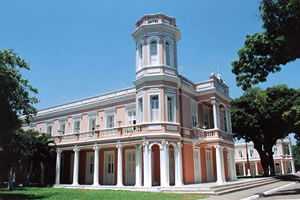
\includegraphics[width=16cm]{figuras/exemplo-1}
		}{
			\Fonte{\citeonline{UFC2012}.}
	}
	\end{figure}
	
    Texto1 texto texto texto texto texto texto texto texto texto texto texto texto texto texto texto texto texto texto texto texto texto texto texto texto texto texto texto texto texto texto texto texto texto texto texto texto texto texto texto texto texto texto texto texto1.

    Texto2 texto texto texto texto texto texto texto texto texto texto texto texto texto texto texto texto texto texto. Texto texto texto texto texto texto texto texto texto texto texto texto texto texto texto texto texto texto texto2.

    Texto3 texto texto texto texto texto texto texto texto texto texto texto texto texto texto texto texto texto texto. Texto texto texto texto texto texto texto texto texto texto texto texto texto texto texto texto texto texto texto3.

    Texto4 texto texto texto texto texto texto texto texto texto texto texto texto texto texto texto texto texto texto. Texto texto texto texto texto texto texto texto texto texto texto texto texto texto texto texto texto texto texto4.

    A Figura \ref{fig:sondas} Texto texto texto texto texto texto texto texto texto texto texto texto texto texto texto texto texto texto texto. Texto texto texto texto texto texto texto texto texto texto texto texto texto texto texto texto texto texto texto3.

	\begin{figure}[h!]
		\centering
		\captionsetup{width=14cm}%Da mesma largura que a figura
		\Caption{\label{fig:sondas} Gráfico da Atmosfera Superior}	
		\UFCfig{}{
			\includegraphics[width=14cm]{figuras/sondas}
		}{
			\Fonte{adaptado da \citeonline{NASA2016}.}}	
	\end{figure}

    Texto5 texto texto texto texto texto texto texto texto texto texto texto texto texto texto texto texto texto texto texto texto texto texto texto texto texto texto texto texto texto texto texto texto texto texto texto texto texto texto texto texto texto texto texto texto5.

    Texto6 texto texto texto texto texto texto texto texto texto texto texto texto texto texto texto texto texto texto texto texto texto texto texto texto texto texto texto texto texto texto texto texto texto texto texto texto texto texto texto texto texto texto texto texto5.

    Texto7 texto texto texto texto texto texto texto texto texto texto texto texto texto texto texto texto texto texto texto texto texto texto texto texto texto texto texto texto texto texto texto texto texto texto texto texto texto texto texto texto texto texto texto texto texto texto texto texto texto texto texto texto texto texto texto texto texto texto texto texto texto texto texto6.

    Evite terminar seções, capítulos e etc com figura. Procure escrever mais.

\section{Inserindo tabelas}\label{sec:tabelas}
    
    A Tabela \ref{tab:exemplo-1}... texto texto texto texto texto texto texto texto texto texto texto texto texto texto texto texto texto texto texto. Texto texto texto texto texto texto texto texto texto texto texto texto texto texto texto texto texto texto texto.
	
	\begin{table}[!h]
	\captionsetup{width=7cm}%Deixe da mesma largura que a tabela
	\Caption{\label{tab:exemplo-1} Um Exemplo de tabela alinhada que pode ser longa ou curta}%
	\IBGEtab{}{%
		\begin{tabular}{ccc}
			\toprule
			Nome & Nascimento & Documento \\
			\midrule \midrule
			Maria da Silva & 11/11/1111 & 111.111.111-11 \\
			Maria da Silva & 11/11/1111 & 111.111.111-11 \\
			Maria da Silva & 11/11/1111 & 111.111.111-11 \\
			\bottomrule
		\end{tabular}%
	}{%
	\Fonte{o autor.}%
	\Nota{esta é uma nota, que diz que os dados são baseados na
		regressão linear.}%
	\Nota[Anotações]{uma anotação adicional, seguida de várias outras.}%
    }
    \end{table}

	%\begin{table}[h!]	
	%	\centering
	%	\Caption{\label{tab:exemplo-1} Exemplo de tabela}	
	%	\UFCtab{}{
	%		\begin{tabular}{cll}
	%			\toprule
	%			Ranking & Exon Coverage & Splice Site Support \\
	%			\midrule \midrule
	%			E1 & Complete coverage by a single transcript & Both splice sites\\
	%			E2 & Complete coverage by more than a single transcript & Both splice sites\\
	%			E3 & Partial coverage & Both splice sites\\
	%			E4 & Partial coverage & One splice site\\
	%			E5 & Complete or partial coverage & No splice sites\\
	%			E6 & No coverage & No splice sites\\
	%			\bottomrule
	%		\end{tabular}
	%	}{
	%	\Fonte{elaborado pelo autor.}
	%}
	%\end{table}

\subsection{Exemplo de subseção} \label{sec:ex_sec}
	
    Texto texto texto texto texto texto texto texto texto texto texto texto texto texto texto texto texto texto texto texto texto texto texto texto texto texto texto texto texto texto texto texto texto texto texto texto texto texto texto texto texto texto texto texto texto.

    %acrlong{DATASUS},\acrlong{DNV},\acrlong{DO},\acrlong{ESF},\acrlong{IBGE},\acrlong{MFC},\acrlong{MI},\acrlong{MS},\acrlong{NV},\acrlong{ODM},\acrlong{OI},\acrlong{OMS},\acrlong{ONU},\acrlong{PNI},\acrlong{PSF},\acrlong{RIPSA},\acrlong{RN},\acrlong{SIM},\acrlong{SINASC},\acrlong{SUS},\acrlong{TMI},\acrlong{TMMFC}


    \begin{alineascomponto}
	    \item Integer non lacinia magna. Aenean tempor lorem tellus, non sodales nisl commodo ut
	    \item Proin mattis placerat risus sit amet laoreet. Praesent sapien arcu, maximus ac fringilla efficitur, vulputate faucibus sem. Donec aliquet velit eros, sit amet elementum dolor pharetra eget
	    \item Integer eget mattis libero. Praesent ex velit, pulvinar at massa vel, fermentum dictum mauris. Ut feugiat accumsan augue, et ultrices ipsum euismod vitae
	    \begin{subalineascomponto}
		    \item Integer non lacinia magna. Aenean tempor lorem tellus, non sodales nisl commodo ut
		    \item Proin mattis placerat risus sit amet laoreet.
	    \end{subalineascomponto}
    \end{alineascomponto}

\subsection{Uso de siglas} \label{sec:siglas}

    Para utilizar siglas, primeiro defina a sigla no arquivo "lista-de-abreviaturas-e-siglas"~ dentro da pasta "1-pre-textuais" com o comando 
    \begin{verbatim}
        \newacronym{ABNT}{ABNT}{Associação Brasileira de Normas Técnicas}
    \end{verbatim}
    Depois chame a sigla com o comando:
    \begin{verbatim}
        \gls{ABNT}
    \end{verbatim}
    Fica assim: \gls{ABNT}. A primeira vez que o comando é usado para uma determinada sigla, aparece o significado por extenso da sigla com a sua abreviação em seguida. A partir da segunda vez que o comando para uma determinada sigla é usado, aparace apenas a sigla. Por exemplo: \gls{ABNT}.  
    
    Veja o código fonte de outros exemplos: Teste de siglas \gls{TEST}, outros exemplos de siglas: \gls{DA}, \gls{MCEG}. 
    Repare que sempre as siglas estão sendo definidas primeiramente no arquivo ``lista-de-abreviaturas-e-siglas''.

	\gls{coerencia}
	\input{2-textuais/3-metodologia}
	\input{2-textuais/4-resultados}
	\input{2-textuais/5-conclusao}
	
	%Elementos pós-textuais	
	\bibliography{3-pos-textuais/referencias}
	\imprimirglossario
	\imprimirapendices
		% Adicione aqui os apendices do seu trabalho
		\input{3-pos-textuais/apendices/apendice-a}
		\input{3-pos-textuais/apendices/apendice-b}
		\input{3-pos-textuais/apendices/apendice-c}
		\input{3-pos-textuais/apendices/apendice-d}
	\imprimiranexos
		% Adicione aqui os anexos do seu trabalho
		\input{3-pos-textuais/anexos/anexo-a}
		\input{3-pos-textuais/anexos/anexo-b}		
	\imprimirindice

\end{document}